\chapter{The State of the Art}

Many researchers are concerned with finding metrics of software quality. The human factor is one of the most significant factor in the development process. Therefore, the related work in  cognitive performance and influences is an important area and related knowledge to find factors in the software development.\\
This chapter provides a summary of their previous research and related work.
\bigbreak
Measuring quality of software projects and gaining information about the progress are valuable information for the software engineers and developers to reflect their performance. The provided feedback helps them to identify their weaknesses and improve their skills or optimize their work patterns \cite{johnson1999leap} \cite{Martin:2008:CCH:1388398}.\\
Also project managers have a great interest in details about the progress and the products quality in order to coordinate the schedules, resources and having an overview about the possible bottlenecks in the project.
Early knowledge about potential problems can help them to target it and make a difference between the success or failure of a software project.
\bigbreak
A good programmer nowadays is described as a person who can solve complicated problems by breaking them down in smaller targeted problems that are easy to understand and to solve. 
\\
Good code is supposed to be clean, easy to read and as simplyfied as possible \cite{johnson1999leap}.
\\
This new approach differs from the early days when programmers tried to find the shortest and most performant solutions. As long as code was using minimal resources it was fine. Less people were working on projects and the open source community was not as important and big as today. A lower computing power in that days made computers unable to handle the complexity that software has today. \\
More people are working together on different parts of complex systems. At the end every part must go hand in hand with all other parts and the code should have a similar structure so that people from one team could possibly also work or help out in another team.
\bigbreak
From a research perspective it is very interesting to get an overview approaches from different years to gain a broader understanding. Thus the following paragraphs will summarize information about code metrics and code quality from several decades.

\section{Software Metrics}
Since the late 1960s, when the software development was in it's beginning, people wanted to measure and produce numbers to characterize code properties. 
The first metrics where used and developed to measure and evaluate the performance of a programmer. Lines of Code (LOC) per month and bugs per thousand lines of code (KLOC) are very simple but efficient ways for examining the productivity, which can be used to for comparison with other programmers or general standards.
\bigbreak
``Software Metrics`` is the term that has been used since more then 30 years.
Today, many metrics are still used to investigate the productivity of the software developers. The amount of bugs in relation to the amount of code, the initiall number of requierements compared to the requierememts at the current point in the project and the effort it takes to fix faults versus the total time the project reqieres \cite{kaner2004software}.\\
The metrics have been a great success in the industry. Most of the big software companies and even smaller ones use metrics, though they are barely used in academia. 
The metrics are created for larger software and scopes. Maintenance and re-factoring is not as important in academia as it is in the industry with commercial software. After all, Software metrics in the industry are primarily used for the management rather than for the development process itself.\\
Industrial software metrics can be used to ensure quality, productivity and can even make predictions of the software quality and software reliability \cite{fenton1999software}.\\
Several researchers investigated and developed approaches to improve the metrics and the results which they are generating. 
Yue Jiang et. al. \cite{jiang2008comparing} from West Virginia University researched methods for improving software quality predictions. They used supervised machine learning algorithms with datasets and focused on improving of the information content of the training data in their research. Their results showed evidence that the biggest differences in the quality of the predictions are generated by the choice of the right software metrics rather than applying different machine learning algorithm. 

\subsection{Summary}
Software metrics are values that indicate the quality and performance in software development. It is more common in project management for measuring the progress and for making predictions rather than for improving the development process and giving feedback to the developers. 


\section{Metrics Measurement and Analysis}
PSP - Personal Software Process is a way to gather data about the Software engineering process and analysis of the information \cite{hayes1997textordfemininethe}.
Over the last decades, the University of Hawaii did a lot of research in PSP and they developed different approaches to bring students to adopt and use it in their projects and even later in their profession as a developer.\\
Their first approach was originally described as ``A Discipline for Software Engineering'' \cite{humphrey1995discipline}. It required the users to keep records about all the metrics by hand. The massive overhead was a high barrier for the students to adopt and keep on working with the PSP. For the best results they needed to write down every compiler error and they had to track the time they were working on their projects and had to stop it for interruptions.\\
In 1998 the University of Hawaii started the Leap research project to provide a PSP with low overhead for the collection and analysis of the data. This generation of PSP was using automated tools which were asking the user for inputting the data. These tools were also able to display information and analyses to the user.
Just a few students adopted the system. The researchers found out that another reason for the reluctant adoption was the constant context switches for the users. Inputting the data during the programming task interrupted and disturbed the ability to focus on the programming tasks \cite{johnson2003beyond}. 
In order to eliminate the adopting barriers, they started the Hackystat project in 2001. Hackystat is an open source framework for automatically gathering all the required metrics by data collection plugins in the development environments of the users. Table \ref{psps} shows the evolution of the PSPs from the University of Hawaii.\\
Plugins, that are installed by the in their programming environments automatically collect the data and forward it to a centralized web service. The web service orders and analyzes the data. If interesting results occur, the webservice sends emails to the developers to inform them about it. The web service also provides a rich visual representation of the data.
All the different approaches to provide feedback about the code lead to improvements in the quality and the ability to estimate software projects. \cite{johnson2001project} 
The Appalachian State University in North Carolina described a different approach. Their goal was to decrease the high attrition rate of computer science students and increase the attraction to get a computer science degree in general.\\
The researchers were monitoring the students software development behavior in order to find good practices for successfully learning programming. For gathering the data of the individual students, they developed a tool called ClockIt. ClockIt allows to, fully automatically, collect the data, analyze it and compare the results with the results from better or more experienced students visually. A web interface provides access to measurements for the student, the course instructor or an administrator.\\
In their results they compared the data of three students out of 75 participants. The students with the best results, an average scoring student and the one with the lowest grade. 
The comparison showed that the best student also spent the most time on the project, but wrote less code than the average scoring student who spend almost as much time. The worst student spend the least time and submitted the smallest amount of code. There was an interesting correlation between the grade and the compilation errors and the amount of compilations that were made. The best student compiled the code more than double as much as the average student and almost 6 times more than the worst student did. \cite{norris2008clockit}

\begin{table}[ht]
  \begin{tabular}{|P{5cm}|P{3cm}|P{3cm}|P{3cm}|}
  \hline
   \textbf{Characteristic}	& \textbf{Generation 1} & \textbf{Generation 2 - Leap} & \textbf{Generation 3 - Hackystat} \\ \hline
	Collection overhead	& High 											& Medium  				& None \\ \hline
	Analysis overhead	& High 											& Low 						& None \\ \hline
	Context switching	& Yes 											& Yes 						& No \\ \hline
	Metrics changes		& Simple 										& Software edits		& Tool dependent \\ \hline
	Adoption barriers		& Overhead, Context-switching 	& Context-switching	& Privacy, Sensor availability \\ \hline
  \end{tabular}
  \newline\newline
  \caption{University of Hawaii - PSPs}\label{psps}
\end{table}

\subsection{Summary}
This section describes the evolution of analyzing software engineering processes. It started with documenting every step by hand up to fully automated plugins that gather and analyzed the data without any work of the developer.
The section ends with an example of a study that was executed with a data collecting and analyzing tool and its results. 


\section{Mobile Data Gathering}
Ferreira, D., et al. \cite{ferreira2015aware} from the University of Oulu, Finland and the Carnegie Mellon University were working on a toolkit for gathering the sensor data from mobile Android devices. They created an extensible framework that could have been used in any Android application at the time when the paper was released. They also released an application for research purposes (the Aware client). The Aware client is extendable with plugins to support more than the pre-installed sensors. By default, the application stores the gathered data on the local hard disk but can also be uploaded to a database.\\
The sensoring is optimized to keep the energy impact as little as possible and not to use more device resources than necessary.
\bigbreak
Another approach in the area of mobile data gathering have been made by University of Science and Technology of China HUI XIONG, Rutgers University in cooperation with Nokia. In order to detect the context of the mobile device, Zhu, Hengshu, et al. \cite{zhu2015mining} were reading the log files of the device. The device logs provide information about location, accelerometers and optical sensor as well as browser history or which apps were used and are automatically recorded by the Android operating system. These information can be used to provide context aware suggestions e.g. for other games or based on the physical location. To read the logged information, the needs to be physically connected computer.\\
The information from the device logs are much richer than the information which can be gathered in an application with the downside, that the device needs to be connected to a computer in order to access the information. A installed application can compute, store and transfer the data  to a remote server from everywhere. The only requirement is access to the internet.

\subsection{Summary} 
This section describes two different approaches of using the mobile phone for gathering the sensor and device data. The first approach is using an application for that purpose while the second research team was reading the device logs which required physical access to the mobile device.


\section{Data Clustering}
In order to give data a meaning it makes sense to cluster in a logical way and make assumptions about the needed features or contexts. 
The article ``Data Clustering: A Review'' \cite{jain1999data} provides a wide overview of different techniques and ways to classify data into groups. They describe a variety of different clustering techniques, all with the goal to find patterns and assign data to a specific category that allows to work it. The clustering can be be distinct between hierarchical and partitional techniques. Different from a hierarchy, the partional methods don't produce a hierarchy but simple partitions. In their paper they describe different techniques for clustering different kinds of data such as image segmentation, object recognition, document retrieval and data mining. Different techniques can be useful for different kinds of applications and therefore no perfect solution for everything is found. 
In another study, researchers from the University of Ouluu, Finland used the data of a wide range of different sensors to detect the context of the user \cite{korpipaa2003bayesian}. They gathered data from a microphone, a three directional accelerometer, thermometer, light sensors and measured the humidity and skin conductivity. 
they were using naive bayesian classifiers to combine the gathered data and correlate them with samples. For example, they recorded the ambients of different environments such as being in an elevator or the sound of a car or conversations. They got the features from their audio files by using algorithms from the MPEG-7 standardized metadata. Different environments have different key features in their ambient, such as constant noise (e.g. tap water) or peaks(e.g. conversation).
Audio was their most valuable information, but for example the humidity was helping to detect very accurate whether the user is in- or outside.
The results of the experiment show a very accurate detection of the correct context in \ref{clustering}. Features like being inside or outside as well as detection whether rock or classical music was played were detected very well. Detection between walking and running or active and still were less accurate.
The combined true positive rate was more than 90\% and the true negative value was over 85\%. Their usage of good test data placing their sensors in a good way helped a lot to get good results. In reality, when users have phones, they carry them in purses, pockets or their hand which makes it much harder to detect the current context.
Context aware computing was already the topic of a great paper in 1995 written by a team from the Columbia University and the Xerox Corporation \cite{schilit1994context}. They describe a context aware system for an office environment. The systems uses the user's location, lightning, communication bandwidth and proximity to other users within the office in order to customize the application functionality depending on the context. This could for example include the displaying of experiment information, when the user is in his lab or showing the calendar when another person is in a close range. It can also be used to create context based reminders for specified locations, time, when seeing specific people or all combined. 

\begin{figure}
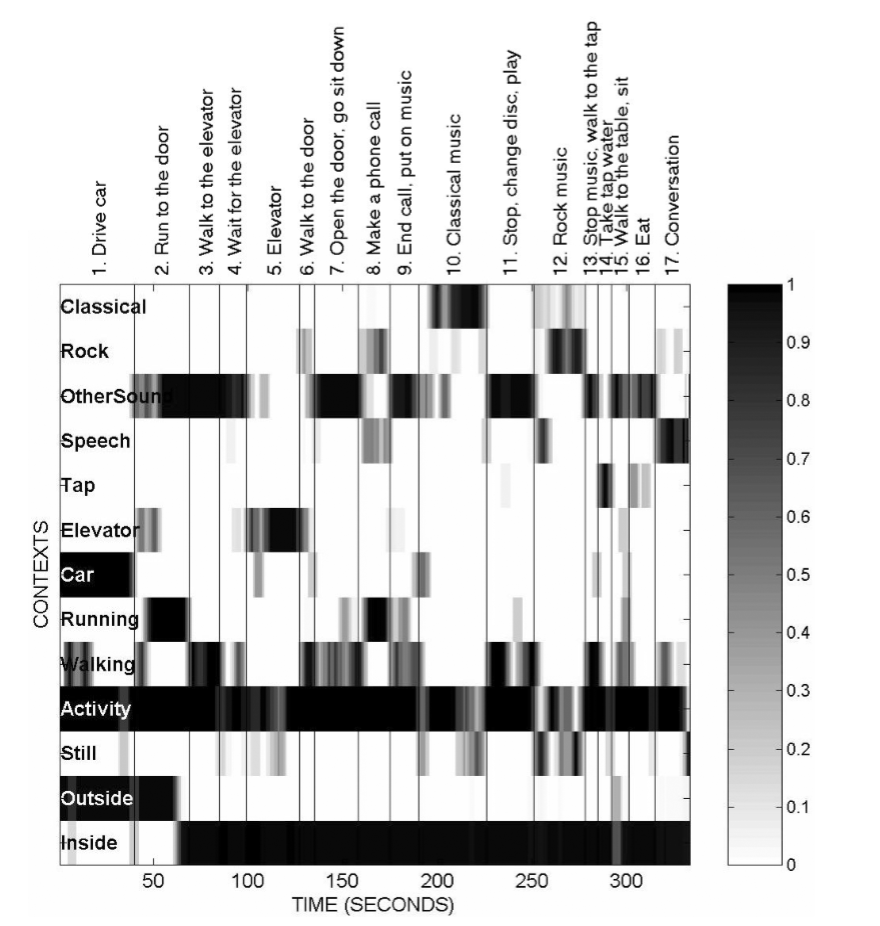
\includegraphics[width=10 cm]{clustering}
\caption{Data Clustering \cite{korpipaa2003bayesian}}\label{clustering}
\vspace{2 mm}
\end{figure}

\FloatBarrier

\subsection{Summary} 
In this sections, approaches and ideas about bringing data into context are described. Clustering techniques are mentioned as well as different approaches to classify the information by comparing them to patterns. Sometimes single sensor-values are enough to be able to cluster properly to identify the meaning of the data. Though, mostly it is the combination of different sensor-values that give more clarity about the context.


\section{Variable Quality Influences}
The majority of software quality is based on the cognitive performance of the software developer and the communication within the team. 
When the single developers write brilliant code, but don't know what the others do or need, the code can't work. On the other hand, the code quality still stay bad even when the development team communicates perfectly but the individual programmers write bad code \cite{moe2010teamwork}. The following sections will provide an overview about the previous research of the individual factors in that area. 

\subsection{Team Communication}
The differences between teams with high cooperating team-members against project teams with less communication have been investigated an discussed by Mary Beth Pinto and Jeffrey K. Pinto \cite{pinto1990project}. They tested the two different groups on performance in tasks and the psychological outcomes.\\ 
Several different factors have been tested and resulted significantly better in the high communicating group. They scored higher in resolving problems, brainstorming, progress review, obtaining information, gaining authorization to perform tasks and in receiving feedback. The low cooperating team did only get a better score in resolving conflicts, which is not surprising as fewer communication already avoid conflicts. 
\bigbreak
The importance of the communication in software teams is gaining more and more attention from companies within the last few years. The companies and teams came up with several ideas to improve the internal communication. 
Agile software engineering methods is the solution for a lot of teams and companies to reach the goal of a better exchange of information within the company. The concept is based on flexibility and responsibility within a software project.\\
Instead of having a the whole project scheduled and structured at the beginning, agile concepts allow to react to problems and new information in a faster way /cite{chow2008survey}. One of the most used and successful methods to work in agile teams is scrum.
\bigbreak
In scrum, the tasks are separated in different phases that are called sprints. A sprint is a short time period in that a defined goal should be reached. This goal can be, for example a feature or a new component. After the sprint the team comes together again and decides about the next sprint and defines the next realitic realizable goals. I this way the team has a lot of responsibility about the project and a lot of freedom how they reach their goals within the sprint period. At the end of each sprint or a defined period, the team comes together for a retrospective to discuss the last sprint/s and how to improve the processes in the next period and if they change some methods such as the daily meeting. The daily meeting is done buy some scrum teams, where every team member summarizes the achievements and problems from the previous day. This meeting can be useful or just wasting time. In Order to find the best working and management patterns the teams can test different methods and discuss them in the retrospective. This dynamic changing and regular feedback is one of the reasons why scrum is used more and more in modern software teams \cite{rising2000scrum} \cite{moe2010teamwork} even with downsides that the company needs to increase the trust in the employees and give up some control \cite{ramesh2006can}.
\bigbreak
Another problem with the communication in teams comes with the increasing globalization and the internet. The ability that and employee can work from every part of the world with an internet connection brings the disadvantages that the software developers do not necessarily sit in the same room anymore or have their working place within a walking distance. 
Also allowing homeoffice for a few days a week is an option that employers provide their employees in order to be a more attractice and family friendly oriented. These changes also requiere new techniques to communicate within the teams. Communication can be done by using video conferences or email. However, both techniques have their disadvantages. A videocall needs to be scheduled and requeres a good internet communication and the problem with emails are the delayed response times and it is too easy for others to ingnore an incoming email\cite{carmel1999global}.\\
One possible solution is chat software which finding their way more and more in the daily communication in software development teams \cite{jarvenpaa1998communication}.\\ 
Slack is the most used tool for chatting at work. The great success in these new way to communicate shows in the rediculous growth. The company Slack is the fastest growing Startup in the world. After just twenty month after its launch in February 2014, already more than 1.7 million people where using Slack  \cite{bercovici2015}.

\subsubsection{Summary} 
This section describes the research in teamwork and communication. I was found that a team with more communication created better results than a team with less communication. \\
In order to improve communication new agile methods such as scrum were introduced. This section also mentioned the problems that employees are not necessarily working in the same office all the time. The latest approaches that deal with this new problems are for example chat software or video calls. 


\subsection{Cognitive Performance}
Looking at the individual programmer, the most important factor is obviously the cognitive performance of the individual person. This section shows the research in the circumstances and influences that can impact the performance in a long or short term. 

\subsubsection{Working Environment}
Improving the perfomance in Software Development can be done in a several different ways. One approach to improve the performance is the optimization of the working environment. Amabile, Teresa M., et al. \cite{amabile1996assessing} wrote about a conceptual model for increasing creativity in the work environment. Five key factors were described. The first two factors were, the encouragement for innovation and creativity as part of the company culture as well as according autonomy or freedom for the employees. Another key described the adequate availability of resources for a project which might affect people psychologically by the feeling to work on a valuable project. Also pressure at work was identified to increase creativity on a balanced level between excessive demands and boring routine. The last key factor in their model described the organizational impediments to creativity which could be caused by internal competitions.
A study was designed to investigate two hypotheses: The influence of the model in high-creative projects vs low-creative projects is expected to be much bigger. As well as obstacles scales are lower in high-creative projects compared to low-creative projects for workload with pressure and organizational impediments.
Both hypotheses had clear result outcomes, which showed that beside the employee's itself, the management can significantly influence the level of creativity and innovation by forming the organization culture. The construction of the teams and definition of the individual roles can have a great impact on the creativity. 

\subsubsection{Context Switching}
Devin G. Pope and Ian Fillmore from the University of Chicago \cite{pope2015impact} inspected correlations in cognitive performance of students and the time between written exams. 
Depending on the schedule of the examinations, students from one year have a different amount of time between exams than students in different years.
As a comparison they name the example of physical performance. If the body has a longer time to recover from one task, it performs the seconds task better compared to a shorter recovery time between these two tasks.\\ 
In this article they compare the scores of the students in their exams and the amount of days between the examination days. 
The study involves information about the students as class(Senior, Junior, Sophomore), Gender and their Race. They all were writing Advanced Placement (AP) Exams in the USA. 
Their results show that a longer break increases the probability that the students pass the exams by 6-8\%. The increasing of the performance is linear up to 10 days.
\bigbreak
As one of the possible reasons for the outcome the researchers names fatigue which is caused by the exhausting task of studying and writing the exam. Another theory is that the last-minute preparations are important for good results but harder to realize when exams are closer together. 
Rogers and Monsell from the University of Cambridge \cite{rogers1995costs} executed an experiment to find out how a context switch can influence the performance on cognitive tasks. It showed that a frequent context or task switching has a negative impact on the error rate and the reaction time of the participants for the tasks they did. Repeating this experiment for three days yielded that the practice has no positive influence on the error rate and thus shows as well that context changing is negatively influencing productivity and performance. 

\subsubsection{Arousal Effects}
The cognitive performance can vary based on the context and the environment. When the body is in a relaxed state, the mind also slows down to save resources. It made sense back in the stone age because thinking was not as important as today. Cognitive performance was mainly needed in dangerous or unusual situations where the heart beat is faster to provide the brain and the muscles with more oxygen and a higher arousal than normally.\\
\bigbreak
Researchers from the Brunel University in the UK showed movie clips to participants in order to invoke different defined moods before the participants had to solve given debugging/coding tests. The results showed improvements in their score after the participants were confronted with high arousal video clips. Low arousal clips affected their performance in a negative way compared to neutral clips \cite{khan2007mood}.\\ 
It is called the Yerkes-Dodson Law, which proclaims that a higher level of arousal leads to better cognitive performance. As caffeine also influences the arousal, it also can be used to boost the cognitive performance and is not just helping to wake up in the morning. Watters, Paul Andrew et. al. \cite{watters1997caffeine} found out that the average caffeine for the best cognitive results is an amount of 400 mg for one person. That is the amount that is contained in ca. 5 espresso shots.
\bigbreak
When an arousal stimmulation can be influencing the performance of a programmer, other factors that are effecting the mood could also have an impact in the quality of the written software. Many people believe that, for example the weather has a strong influence in the daily mood of a person. Certainly, Denissen, Jaap JA, et al. \cite{denissen2008effects} found out that the sunshine alone actually has no notable effect in the mood of the most of the people. Certainly, some individuals have a so called seasonal affective disorder (SAD). Their mood is indeed strong being affected by the seasons with fall and winter depressions.\\ 
However, they found significant correlations between sunlight, air pressure and precipitation on the tiredness of the participants.
A reason for the influence of sunlight could be vitamin D3. The most of it is obtained through exposure to sunlight and it changes the level of serotonin which was found to be partly responsible for the mood of a human.

\subsection{Activity} 
The researchers Hillman C, et al. \cite{hillman2008smart} found evidence for positive effects of regular activity on cognition and brain functionality for human and animals. They found that especially aerobic has a strong positive influence. 
A meta analysis showed that children who were physically active were better in all tested categories (IQ, perceptual skills, verbal tests, math, memory, academic readiness and others). 
These effects were also shown in other age groups but were the strongest for children. Older people who were active during their life showed a smaller risk of Alzheimer and Dementia. 

\subsubsection{Diet}
A very different, but probably the most important factor in the long term cognitive performance are temporary diets and the consumed food during the lifetime. The human brain needs good fuel to run properly. A wrong diet can strongly influence the incidences of cognitive problems as well as healthy food can positively influence healthy ageing \cite{spencer2008food}.\\
Some eatables demonstrated positive effects on the mental performance when they were containing flavonoids like for example grapes, tea, cocoa and blueberries. 
Different to the previous influences, the diet and the lifestyle are less obvious in their consequences. Their impact is slowly showing over several years and it's hard to prove their effects and that they are the influencing factors.\\
Studies on several mammalian species have shown that food which is rich of flavonoids have beneficial effects on memory and learning, with the ability to support neurons and protecting them again stress-induced injury.
These foods also decreases the chances of Alzheimer and dementia. Other studies have shown that flavonoid-rich groceries improves the blood circulation and correlates with the growing of new hippocampal cells. These cells are located in the brain region that is identified to be responsible for the memory.

\subsubsection{Summary} 
This section is about the different influences in the cognitive performance. Starting with the influences of the working environment created by the company with the stress and interest it creates with the projects itself as well as motivation and creativity by giving employees the chances to share their ideas and feel valuable. The nest part investigates the problem and the lower performance that occur when people switch during different tasks and contexts. Afterwards the work of influence of arousal in cognitive performance is summarized and the section end with the influences of physical activity and the diet and the food that has positive impacts. 